      
               
                \begin{ledgroupsized}[r]{120mm}
                \footnotesize 
                \pstart                
                \noindent\textbf{\"{U}berlieferung:}   
                \pend
                \end{ledgroupsized}
            
              
                            \begin{ledgroupsized}[r]{114mm}
                            \footnotesize 
                            \pstart \parindent -6mm
                            \makebox[6mm][l]{\textit{L}}Konzept: LH XXXVII 3 Bl. 128\textendash129. 1 Bog. 2\textsuperscript{o}. 2 S. zweispaltig auf Bl 128. Die verbleibenden Seiten zu N. 49\raisebox{-0.5ex}{\notsotiny 4} geh\"{o}rig. Die Marginalie fig. 1. auf Bl. 128 r\textsuperscript{o} verweist auf \textit{[Fig. 2]} N. 49\raisebox{-0.5ex}{\notsotiny 3}. Das vorliegende St\"{u}ck ist daher sp\"{a}ter entstanden. In der rechten unteren Ecke von Bl. 128 v\textsuperscript{o} hat sich Leibniz mit der Bemerkung \glqq Recherche'' einen Hinweis auf N.~51 notiert.\\Cc 2, Nr. 491 A tlw. \pend
                            \end{ledgroupsized}
                \vspace*{8mm}
                \pstart 
                \normalsize
           \selectlanguage{french}\begin{center}[128 r\textsuperscript{o}] \edlabel{uni128r1}\textso{DE L'UNION DES CORPS,}\\PURGEZ D'AIR; \edtext{}{\lemma{}\xxref{uni128r1}{uni128r1}\Afootnote{\textso{DE L'UNION DES CORPS} \textit{doppelt unterstrichen}}} \edtext{QUI SE TROUUENT JOINTS}{\lemma{}\Afootnote{ \textit{ (1) }\ SOUTEN\"{U}E \textit{ (2) }\ QUI SE TROUUENT JOINTS \textit{ erg.} \textit{ L}}} PAR\\UNE PRESSION DIFFERENTE\\DE CELLE DE L'ATMOSPHERE.\rule[-4mm]{0mm}{4mm}\end{center}\textso{Phenomenes, ou Experiences toutes faites.}\edtext{}{\lemma{}\Afootnote{\textso{Phenomenes, ou Experiences toutes faites} \textit{doppelt unterstrichen}}}
           \textso{Phenomene 1.} Les liqueurs\protect\index{Sachverzeichnis}{liqueur} ne s'\'{e}coulent pas d'un tuyau \'{e}troit, ouuert par un bout seulement, quoyque le tuyau soit renvers\'{e}.\pend \pstart \textso{Phenom. 2.} Pourveu que la hauteur de la liqueur\protect\index{Sachverzeichnis}{liqueur} ne soit pas trop grande, car il y a des hauteurs determin\'{e}es selon l'espece de la liqueur\protect\index{Sachverzeichnis}{liqueur}, (\`{a} raison reciproque de la pesanteur) qui la font tomber. Comme par exemple l'eau ne passe pas, de beaucoup, 30 pieds, ny le Mercure\protect\index{Sachverzeichnis}{mercure} 27 pouces. %\\@@@INSERTION AUSKOMMENTIERT@@@\\ 
           \edtext{Tout cela s'entend l'experience estant faite dans l'air ordinaire, avec des liqueurs quand elles sont encor dans leur constitution naturelle, sans estre purgez d'air. Comme elle a estoit faite par \textso{Galilaei} avec de l'eau, et par \textso{Torricelli} avec du Mercure.}{\lemma{pouces.}\Afootnote{ \textit{ (1) }\ Tout cela s'entend l'experience estant faite \textbar\ dans l'air  \textit{ (1) }\ libre  \textit{ (2) }\ ordinaire \textit{ erg.} \textbar\ avec des liqueurs dans leur constitution naturelle; par \textso{Galilei} avec de l'eau, et par \textso{Torricelli} avec du Mercure. \textit{ (2) }\  Tout cela [...] du Mercure. \textit{ erg.} \textit{ L}}}
           \pend \pstart \textso{Phenom. 3.} Monsieur de Guericke\protect\index{Namensregister}{\textso{Guericke} (Gerickius, Gerick.), Otto v. 1602\textendash 1686} ayant trouu\'{e} moyen \edtext{de}{\lemma{Monsieur}\Afootnote{\textbar\ de \textit{ erg.}  \textbar\ Guericke \textit{ L}}} tirer l'air d'un Recipient d'une notable grandeur \edtext{par une pompe\protect\index{Sachverzeichnis}{pompe}}{\lemma{}\Afootnote{par une pompe\protect\index{Sachverzeichnis}{pompe} \textit{ erg.} \textit{ L}}}; on \edtext{tacha}{\lemma{on}\Afootnote{ \textit{ (1) }\ s'avisa \textit{ (2) }\ tacha \textit{ L}}} de faire l'experience de la suspension des liqueurs\protect\index{Sachverzeichnis}{liqueur}, dans le Vuide\protect\index{Sachverzeichnis}{vide}.\footnote{\textit{In der rechten Spalte als Platzhalter für fig. 1}: fig. 1.} Et pour c\'{e}t effect, le matras \edtext{}{\lemma{matras}\Afootnote{ \textbar\ ou la phiole \textit{ erg. u.}\  \textit{ gestr.}\ \textbar\ \textit{A-CD} \textit{ L}}} \edtext{\textit{A-CD} dans la fig. 1.  estant plein}{\lemma{\textit{A-CD}}\Afootnote{ \textit{ (1) }\ estant rempli \textit{ (2) }\ dans [...] plein \textit{ L}}} d'eau et renvers\'{e} de sorte, que le bout ouuert \textit{A}, trempast dans l'eau du vase \textit{F}, rempli jusque en \textit{A} on couurit le tout du verre ou Recipient \textit{E} et on fit jo\"{u}er la pompe\protect\index{Sachverzeichnis}{pompe}; par le moyen de laquelle la pluspart de l'air estant sortie du Recipient \textit{E}, le matras se vuida\edtext{}{\lemma{}\Afootnote{vuida  \textbar\ entierement \textit{ gestr.}\ \textbar\ , et \textit{ L}}}, et le vase \textit{F} se remplit \`{a} proportion de sa grandeur, ou de celle du matras; \edtext{sans que la liqueur\protect\index{Sachverzeichnis}{liqueur} eût demeur\'{e} suspend\"{u}e, qu'\`{a} proportion de l'air qui estoit rest\'{e} dans le Recipient.}{\lemma{matras}\Afootnote{\textbar~\textbar~, ou de la phiole \textit{ gestr.}\ \textbar\  ; sans que la liqueur\protect\index{Sachverzeichnis}{liqueur}  \textit{ (1) }\ demeurât \textit{ (2) }\ eût [...] Recipient. \textit{ erg.}~\textbar\ \textit{ L}}}\pend     
           \pstart \textso{Phenomen. 4.} Mais comme l'eau \edtext{qu'on a}{\lemma{}\Afootnote{qu'on a \textit{ erg.} \textit{ L}}} laiss\'{e} quelque temps dans le vuide fait quantit\'{e} de petites bulles d'air et s'en purge enfin par ce moyen \edtext{pour un temps assez long}{\lemma{}\Afootnote{pour un temps assez long \textit{ erg.} \textit{ L}}}, \textso{Monsieur Huguens}\protect\index{Namensregister}{\textso{Huygens} (Hugenius, Vgenius, Hugens, Huguens), Christiaan 1629\textendash 1695} trouua, que l'eau purg\'{e}e ne tombe pas du matras,\edtext{}{\lemma{}\Afootnote{matras,  \textbar~ou de la phiole \textit{ erg. u.}\  \textit{ gestr.}\ \textbar\ \textit{CD} \textit{ L}}} \textit{CD} quoyque on tire l'air du Recipient \textit{E}.\edtext{}{\lemma{\textit{E}.}\Bfootnote{\textsc{Chr. Huygens, }\cite{00062}\textit{Extrait d'une lettre}, \textit{JS} (1672), S.~134 (\textit{HO} VII, S.~202).}}\pend 
           \pstart \textso{Phenom. 5.} Sinon, quand le tuyau a receu quelque choc considerable ce que \textso{Monsieur de Guericke}\protect\index{Namensregister}{\textso{Guericke} (Gerickius, Gerick.), Otto v. 1602\textendash 1686} a remarqu\'{e} \edtext{aussi,}{\lemma{aussi,}\Bfootnote{Experimente dieser Art sind von Guericke nicht überliefert.}}\pend 
           \pstart \textso{Phenom. 6.} ou quand une bulle d'air estant n\'{e}e au bas du matras \textit{A} ou qu'on a fait entrer par l\`{a} dans le matras, s'enflant et grossissant peu \`{a} peu, se d\'{e}tache de la superficie interieure du verre, et montant par sa legeret\'{e}, arrive \`{a} une certaine hauteur determin\'{e}e \textit{B} dont elle s'\'{e}tend en haut, subitement, et occupant tout l'espace \textit{B-CD} fait tomber l'eau du matras jusqu'\`{a} \textit{B}. \edtext{La hauteur de l'eau \textit{FB} outre son niveau \textit{F},}{\lemma{\textit{B.}}\Afootnote{ \textit{ (1) }\ La hauteur   \textbar\ de l'eau outre son niveau \textit{ erg.}\ \textbar\  \textit{FB} \textit{ (2) }\ La [...] \textit{F}, \textit{ L}}} estant celle, que le peu d'air qui reste dans le Recipient, peut soûtenir par son Ressort, la force duquel determine le point \textit{B}\edtext{, \`{a} ce que \textso{Mons. Huguens a}\protect\index{Namensregister}{\textso{Huygens} (Hugenius, Vgenius, Hugens, Huguens), Christiaan 1629\textendash 1695} observ\'{e}.}{\lemma{}\Afootnote{, \`{a} ce que \textso{Mons. Huguens }\protect\index{Namensregister}{\textso{Huygens} (Hugenius, Vgenius, Hugens, Huguens), Christiaan 1629\textendash 1695}a observ\'{e}. \textit{ erg.} \textit{ L}}}\edtext{}{\lemma{observ\'{e}.}\Bfootnote{\textsc{Chr. Huygens}, \cite{00062}a.a.O., S.~135 (\textit{HO} VII, S.~202f.).}}\pend 
% Zeitz auskommentiert            \begin{center}
%           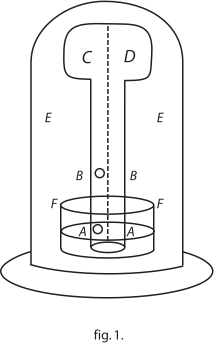
\includegraphics[width=0.4\textwidth]{images/37_3_128r}
%           \end{center}
           \pstart \textso{Phenom. 7.} \textso{Monsieur Boyle}\protect\index{Namensregister}{\textso{Boyle} (Boylius, Boyl., Boyl), Robert 1627\textendash 1691} \edtext{s'avisa de faire le}{\lemma{\textso{Boyle}}\Afootnote{ \textit{ (1) }\ s'avisa de faire le \textit{ (2) }\ trouua moyen de faire le \textit{ (3) }\ s'avisa de faire le \textit{ L}}} même avec du Mercure\protect\index{Sachverzeichnis}{mercure}, purg\'{e} d'air, hors du \edtext{Recipient.}{\lemma{Recipient.}\Bfootnote{\mbox{\textsc{R. Boyle},} \cite{00015}\textit{New experiments physico-mechanicall}, Oxford 1660, Experiment 17, S.~106\textendash129 (\textit{BW} I, S.~192\textendash201).}} Car comme l'eau ordinaire (bien que d'une petite pesanteur), tombe dans le Recipient \'{e}puis\'{e}, parce que l'obstacle de l'air en est ost\'{e}; de même le Mercure\protect\index{Sachverzeichnis}{mercure} ordinaire, tombe dans l'air libre, parce que sa pesanteur est grande: Mais comme l'eau purg\'{e}e ne tombe pas